\section{Phase one}
To execute the first phase of the approach described in Section \ref{sec:first_phase},  we partition the previously described meeting room into a $1m \times 1m$ grid and place beacons as described using painter's tape.%Supervisor requests EXACT setup
To collect measurements for the creation of the map, a person holding a Samsung Galaxy A53 5G phone, with the application described in Section 2 installed and running, traverses systematically through the room and stops at the intersection of each grid line to collect data. 
We will refer to this person as the \textit{collector}.
With the app, it is possible to perform measurements from any number of selected beacons and append a label to the measurements.
In this experiment, the collector selects all beacons and is responsible for the correct collection and labeling of each cell.
\begin{figure}[h]
    \centering
    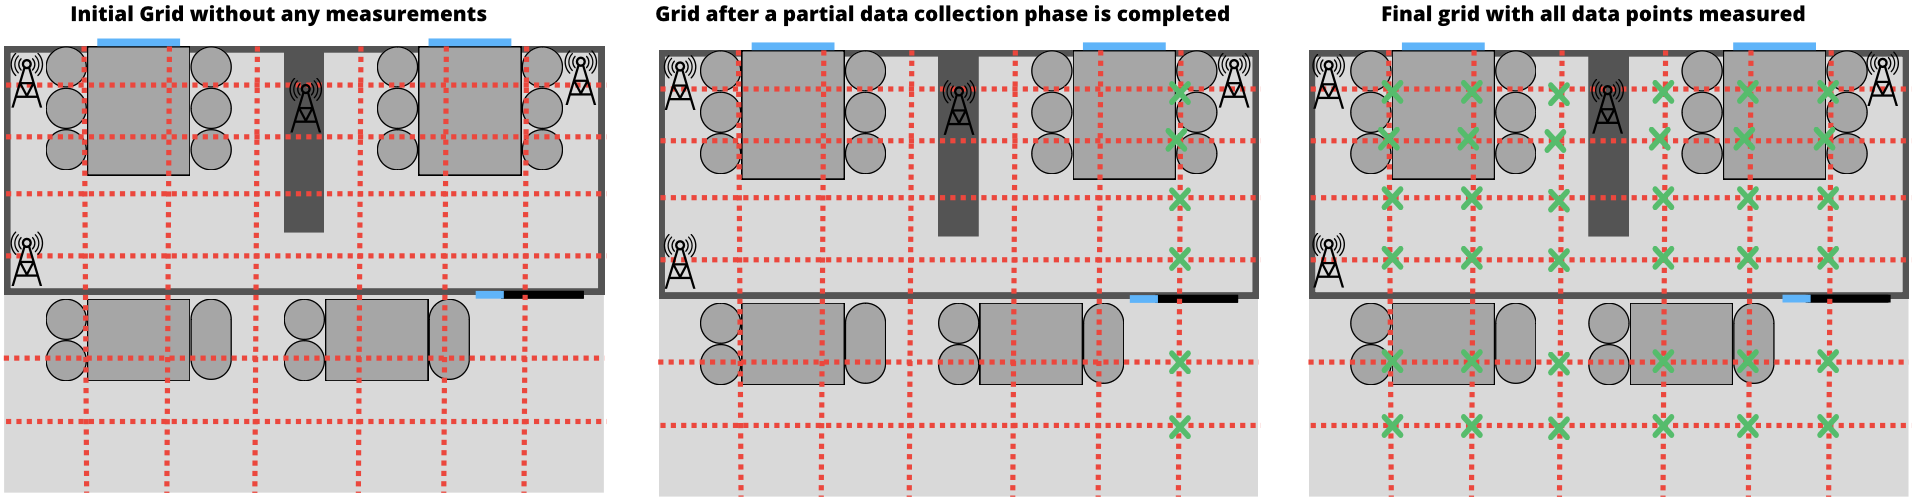
\includegraphics[width=\textwidth]{images/experiment_map_creation.png}
    \caption{A sketch of the meeting room partitioned into a grid decorated with beacon placements (red antenna) and measurement locations (circles with letters). The figure how the measurements are collected systematically in the meeting room.}
    \label{fig:experiment_map_creation}
\end{figure}
When the collector stops at the intersection of two grid-lines, they can press a button in the app, which starts measuring after five seconds.
The phone provides auditory feedback when it has collected enough measurements for the requirements described in Section \ref{sec:first_phase} to be fulfilled.
When the information for measurement has been computed and stored on the phone, the collector is informed auditorily and continues to the next intersection in the grid. 
During the measurement the phone is kept in roughly the same height.
Measurements are collected in a setup using 4 beacons, as depicted in Figure \ref{fig:experiment_map_creation}.
The map creation process was done during out-of-office hours to ensure that the datapoint collected to create the map was collected with a minimum of background signal noise.

